\documentclass[aps,prl,preprint]{revtex4-2}
\usepackage{amsmath}
\usepackage{physics}
\usepackage{bm}
\usepackage{cancel}
\usepackage{graphicx}

\bibliographystyle{apsrev4-2}


\begin{document}
\title{Low flow state}
\author{Jason He}
\affiliation{Department of Physics, Northwestern University, Evanston, IL, US}
\date{July 2025}

% \maketitle

\section{Introduction}
In cylindrical coordinates, we have
\begin{align}
    \begin{pmatrix}
        \eta_r \\ \eta_\phi
    \end{pmatrix}
     = \begin{pmatrix}
         \cos{\phi} & \sin{\phi} \\
         -\sin{\phi} & \cos{\phi}
     \end{pmatrix}
     \begin{pmatrix}
         \eta_x \\ \eta_y
     \end{pmatrix}
\end{align}
and
\begin{align}
    \begin{pmatrix}
        \partial_r \\ \frac{1}{r}\partial_\phi
    \end{pmatrix}
     = \begin{pmatrix}
         \cos{\phi} & \sin{\phi} \\
         -\sin{\phi} & \cos{\phi}
     \end{pmatrix}
     \begin{pmatrix}
         \partial_x \\ \partial_y
     \end{pmatrix}
\end{align}
In bulk, for the two time-reversed ground states,
\begin{align}
    (\eta^\text{bulk}_x, \eta^\text{bulk}_y) = \eta_0(1, \pm i)\\
    (\eta^\text{bulk}_r, \eta^\text{bulk}_\phi) = e^{\pm i\phi}\eta_0(1, \pm i)
\end{align}

In GL theory, the order parameter is determined by minimizing the free energy functional
\begin{align}
    F[\bm{\eta}]=\int\dd[3]r\left(f_{\text{bulk}}+f_{\text{grad}}\right)
\end{align}
where
\begin{align}
    f_{\text{bulk}}[\bm{\eta}]=&\alpha\bm{\eta}\vdot\bm{\eta}^*
    +\beta_1(\bm{\eta}\vdot\bm{\eta}^*)^2
    +\beta_2|\bm{\eta}\vdot\bm{\eta}|^2,
\end{align}
and
\begin{align}
    f^{\text{Car}}_{\text{grad}}[\bm{\eta}]=\kappa_1(\partial_i\eta_j)(\partial_i\eta_j)^*
    +\kappa_2(\partial_i\eta_i)(\partial_j\eta_j)^*
    +\kappa_3(\partial_i\eta_j)(\partial_j\eta_i)^*
\end{align}
In cylindrical basis, we have $\partial_i^\text{Car}=R_{ik}\partial_k$
and $\eta_j^\text{Car}=R_{jl}\eta_l$, where $R_{ij}$ is the 2d rotational matrix.
The form of the bulk free energy term doesn't change.
The gradient term becomes
\begin{align}
    f^{\text{Cyl}}_{\text{grad}}[\bm{\eta}]=&\kappa_1(\partial_i\eta_j)(\partial_i\eta_j)^*
    +\kappa_2(\partial_i\eta_i)(\partial_j\eta_j)^*
    +\kappa_3(\partial_i\eta_j)(\partial_j\eta_i)^*\nonumber\\
    &+\frac{2}{r}\Re{
    \kappa_1\left(\eta_r^*\frac{\partial_\phi}{r}\eta_\phi
    -\eta_\phi^*\frac{\partial_\phi}{r}\eta_r\right)
    +\kappa_2\eta_r^*\partial_j\eta_j
    +\kappa_3\left(\eta_r^*\frac{\partial_\phi}{r}\eta_\phi
    -\eta_\phi^*\partial_r\eta_\phi\right)}\nonumber\\
    &+\frac{1}{r^2}\left[\kappa_1\eta^*_j\eta_j
    +(\kappa_2+\kappa_3)\eta_r^*\eta_r\right].
\end{align}
Take the $\kappa_1$ term for example, note that $R_{ij}R_{ik}=R^T_{ji}R_{ik}=\delta_{jk}$
\begin{align}
    &(\partial_i^{\text{Car}}\eta_j^{\text{Car}})(\partial_i^{\text{Car}}\eta_j^{\text{Car}})^*\\
    =&\bigg[R_{ik}\partial_k(R_{jl}\eta_l)\bigg]\bigg[R_{im}\partial_m(R_{jn}\eta_n^*)\bigg]\\
    =&\bigg[\partial_k(R_{jl}\eta_l)\bigg]\bigg[\partial_k(R_{jn}\eta_n^*)\bigg]\\
    =&\bigg[(\partial_kR_{jl})\eta_l + R_{jl}(\partial_k\eta_l)\bigg]
    \bigg[(\partial_k R_{jn})\eta_n^* + R_{jn}(\partial_k\eta_n^*)\bigg]\\
    =&(\partial_k R_{jl})\eta_l (\partial_k R_{jn})\eta_n^*
    +(\partial_k R_{jl})\eta_l R_{jn}(\partial_k\eta_n^*)
    +R_{jl}(\partial_k\eta_l) (\partial_k R_{jn})\eta_n^*
    +R_{jl}R_{jn}(\partial_k\eta_l)(\partial_k \eta_n^*)\nonumber
\end{align}
Note that $\partial_r R(\phi)=0$, $\partial_\phi R(\phi)=R(\phi)R(\pi/2)=R(\pi/2)R(\phi)$.
Finally we have
\begin{align}
    &(\partial_i^{\text{Car}}\eta_j^{\text{Car}})(\partial_i^{\text{Car}}\eta_j^{\text{Car}})^*\\
    =&\frac{1}{r^2}\eta_l\eta_l^*
    +\frac{1}{r}R^{\pi/2}_{nl}\eta_l\left(\frac{\partial_\phi}{r}\eta_n^*\right)
    +\frac{1}{r}R^{\pi/2}_{ln}\eta_n^*\left(\frac{\partial_\phi}{r}\eta_l\right)
    + (\partial_k\eta_l)(\partial_k \eta_l)^*\\
    =&\frac{1}{r^2}\eta_l\eta_l^*
    +\frac{2}{r}\Re{R^{\pi/2}_{ln}\eta_n^*\left(\frac{\partial_\phi}{r}\eta_l\right)}
    +(\partial_k\eta_l)(\partial_k \eta_l)^*\\
    =&\frac{1}{r^2}\eta_l\eta_l^*
    +\frac{2}{r}\Re{\eta_r^*\frac{\partial_\phi}{r}\eta_\phi - \eta_\phi^*\frac{\partial_\phi}{r}\eta_r}
    +(\partial_k\eta_l)(\partial_k \eta_l)^*
\end{align}
Similarly, for the $\kappa_2$ terms, we have
\begin{align}
    &(\partial_i^{\text{Car}}\eta_i^{\text{Car}})(\partial_j^{\text{Car}}\eta_j^{\text{Car}})^*\\
    =&\bigg[R_{ik}\partial_k(R_{il}\eta_l)\bigg]\bigg[R_{jm}\partial_m(R_{jn}\eta_n^*)\bigg]\\
    =&\bigg[R_{ik}(\partial_k R_{il})\eta_l + R_{ik}R_{il}(\partial_k\eta_l)\bigg]
    \bigg[R_{jm}(\partial_m R_{jn})\eta_n^* + R_{jm}R_{jn}(\partial_m\eta_n^*)\bigg]\\
    =&\bigg[\frac{1}{r}\eta_r + \partial_k\eta_k\bigg]\bigg[\frac{1}{r}\eta_r^* + \partial_m\eta_m^*\bigg]\\
    =&\frac{1}{r^2}\eta_r\eta_r^* + \frac{2}{r}\Re{\eta_r^*\partial_k\eta_k}
    +(\partial_k\eta_k)(\partial_m \eta_m)^*
\end{align}
For the $\kappa_3$ terms, we have
\begin{align}
    &(\partial_i^{\text{Car}}\eta_j^{\text{Car}})(\partial_j^{\text{Car}}\eta_i^{\text{Car}})^*\\
    =&\bigg[R_{ik}\partial_k(R_{jl}\eta_l)\bigg]\bigg[R_{jm}\partial_m(R_{in}\eta_n^*)\bigg]\\
    =&\bigg[R_{ik}(\partial_k R_{jl})\eta_l + R_{ik}R_{jl}(\partial_k\eta_l)\bigg]
    \bigg[R_{jm}(\partial_m R_{in})\eta_n^* + R_{jm}R_{in}(\partial_m\eta_n^*)\bigg]\\
    =&R_{ik}(\partial_k R_{jl})\eta_l R_{jm}(\partial_m R_{in})\eta_n^*
    + R_{ik}(\partial_k R_{jl})\eta_l R_{jm}R_{in}(\partial_m\eta_n^*)\nonumber\\
    &+ R_{ik}R_{jl}(\partial_k\eta_l) R_{jm}(\partial_m R_{in})\eta_n^*
    + R_{ik}R_{jl}(\partial_k\eta_l) R_{jm}R_{in}(\partial_m\eta_n^*)\\
    =&\frac{1}{r^2}R^{\pi/2}_{\phi l}\eta_l R^{\pi/2}_{\phi n}\eta_n^*
    +\frac{1}{r}R^{\pi/2}_{ml}\eta_l(\partial_m\eta_\phi^*)
    +\frac{1}{r}R^{\pi/2}_{kn}\eta_n^*(\partial_k\eta_\phi)
    +(\partial_k\eta_l)(\partial_l \eta_k)^*\\
    =&\frac{1}{r^2}\eta_r\eta_r^* + \frac{2}{r}\Re{R^{\pi/2}_{kn}\eta_n^*(\partial_k\eta_\phi)}
    + (\partial_k\eta_l)(\partial_l \eta_k)^*\\
    =&\frac{1}{r^2}\eta_r\eta_r^* + \frac{2}{r}\Re{\eta_r^*\frac{\partial_\phi}{r}\eta_\phi - \eta_\phi^*\partial_r\eta_\phi}
    + (\partial_k\eta_l)(\partial_l \eta_k)^*
\end{align}
So the free energy density is
\begin{align}
    f_{\text{bulk}}[\bm{\eta}]=&\alpha\bm{\eta}\vdot\bm{\eta}^*
    +\beta_1(\bm{\eta}\vdot\bm{\eta}^*)^2
    +\beta_2|\bm{\eta}\vdot\bm{\eta}|^2,
\end{align}
and
\begin{align}
    f^{\text{Cyl}}_{\text{grad}}[\bm{\eta}]=&\kappa_1(\partial_i\eta_j)(\partial_i\eta_j)^*
    +\kappa_2(\partial_i\eta_i)(\partial_j\eta_j)^*
    +\kappa_3(\partial_i\eta_j)(\partial_j\eta_i)^*\nonumber\\
    &+\frac{2}{r}\Re{
    \kappa_1\left(\eta_r^*\frac{\partial_\phi}{r}\eta_\phi
    -\eta_\phi^*\frac{\partial_\phi}{r}\eta_r\right)
    +\kappa_2\eta_r^*\partial_j\eta_j
    +\kappa_3\left(\eta_r^*\frac{\partial_\phi}{r}\eta_\phi
    -\eta_\phi^*\partial_r\eta_\phi\right)}\nonumber\\
    &+\frac{1}{r^2}\left[\kappa_1\eta^*_j\eta_j
    +(\kappa_2+\kappa_3)\eta_r^*\eta_r\right].\label{fgrad}
\end{align}

\section{Euler-Lagrange equations}

The GL differential equations $\delta F/\delta\eta_k^*=0$.

If we do the functional variation of the free energy in cylindrical basis, we will get
\begin{align}
    \alpha\eta_k+2(\beta_1\eta_i\eta_i^*\eta_k
    +\beta_2\eta_i^2\eta_k^*)-\left(\kappa_1\partial_i^2\eta_k
    +\kappa_2\partial_k\partial_i\eta_i
    +\kappa_3\partial_j\partial_k\eta_j\right)\nonumber\\
    -\frac{1}{r}\left[(2\kappa_1+\kappa_3)\frac{\partial_\phi}{r}
    \left(\eta_r\delta_{k\phi}-\eta_\phi\delta_{kr}\right)+\kappa_1\partial_r\eta_k
    +(\kappa_2+\kappa_3)\partial_k\eta_r\right]\nonumber\\
    +\frac{1}{r^2}[\kappa_1\eta_k+(\kappa_2+\kappa_3)\eta_r\delta_{kr}]
    =0.
\end{align}
For the $\kappa_1$ term in first line of Eq. (\ref{fgrad})
\begin{align}
    F\sim\iint (\partial_i\eta_j)(\partial_i\eta_j)^* r\dd\phi\dd r
    =&\qq{surface term} - \iint \eta_j^*\partial_i(r\partial_i\eta_j) \dd\phi\dd r\\
    =&\qq{surface term} - \iint \eta_j^*\frac{1}{r}\partial_i(r\partial_i\eta_j) r\dd\phi\dd r
\end{align}
the corresponding functional variation is
\begin{align}
    \delta F/\delta\eta_k^*\sim-\frac{1}{r}\partial_i(r\partial_i\eta_k)
    =-\frac{1}{r}(\partial_i r)(\partial_i\eta_k)-\partial_i^2\eta_k
    =-\frac{1}{r}\partial_r\eta_k - \partial_i^2\eta_k
\end{align}
For the $\kappa_2$ term in first line of Eq. (\ref{fgrad})
\begin{align}
    \delta F/\delta\eta_k^*\sim-\frac{1}{r}\partial_k(r\partial_i\eta_i)
    =-\frac{1}{r}(\partial_k r)(\partial_i\eta_i)-\partial_k\partial_i\eta_i
    =-\delta_{kr}\frac{1}{r}\partial_i\eta_i - \partial_k\partial_i\eta_i
\end{align}
For the $\kappa_3$ term in first line of Eq. (\ref{fgrad})
\begin{align}
    \delta F/\delta\eta_k^*\sim-\frac{1}{r}\partial_i(r\partial_k\eta_i)
    =-\frac{1}{r}(\partial_i r)(\partial_k\eta_i)-\partial_i\partial_k\eta_i
    =-\frac{1}{r}\partial_k\eta_r - \partial_i\partial_k\eta_i
\end{align}
For the $\kappa_1$ term in second line of Eq. (\ref{fgrad})
\begin{align}
    F\sim\iint\frac{1}{r}\left(
    \eta_r^*\frac{\partial_\phi}{r}\eta_\phi
    -\eta_\phi^*\frac{\partial_\phi}{r}\eta_r
    + \eta_r\frac{\partial_\phi}{r}\eta_\phi^*
    -\eta_\phi\frac{\partial_\phi}{r}\eta_r^*
    \right)r\dd\phi\dd r
\end{align}
the corresponding functional variation is
\begin{align}
    \delta F/\delta\eta_k^*\sim\frac{1}{r}\left(
    2\delta_{kr}\frac{\partial_\phi}{r}\eta_\phi - 2\delta_{k\phi}\frac{\partial_\phi}{r}\eta_r\right)
\end{align}
The $\kappa_2$ term in second line of Eq. (\ref{fgrad}) is
\begin{align}
    F\sim\iint\frac{1}{r}\left(
    \eta_r^*\partial_j\eta_j + \eta_r\partial_j\eta_j^*
    \right)r\dd\phi\dd r
\end{align}
the corresponding functional variation is
\begin{align}
    \delta F/\delta\eta_k^*\sim\frac{1}{r}\left(
    \delta_{kr}\partial_j\eta_j - \partial_k\eta_r\right)
\end{align}
The $\kappa_3$ term in second line of Eq. (\ref{fgrad}) is
\begin{align}
    F\sim\iint\frac{1}{r}\left(
    \eta_r^*\frac{\partial_\phi}{r}\eta_\phi - \eta_\phi^*\partial_r\eta_\phi
    + \eta_r\frac{\partial_\phi}{r}\eta_\phi^* - \eta_\phi\partial_r\eta_\phi^*
    \right)r\dd\phi\dd r
\end{align}
the corresponding functional variation is
\begin{align}
    \delta F/\delta\eta_k^*\sim\frac{1}{r}\left(
    \delta_{kr}\frac{\partial_\phi}{r}\eta_\phi
    \cancel{- \delta_{k\phi}\partial_r\eta_\phi}
    - \delta_{k\phi}\frac{\partial_\phi}{r}\eta_r
    \cancel{+ \delta_{k\phi}\partial_r\eta_\phi}\right)
\end{align}
Adding all these contributions together, we can get the GL equations in cylindrical basis.

In cartesian basis the GL equations are
\begin{align}
    \alpha\eta_k+2(\beta_1\eta_i\eta_i^*\eta_k
    +\beta_2\eta_i^2\eta_k^*)-\left(\kappa_1\partial_i^2\eta_k
    +\kappa_2\partial_k\partial_i\eta_i
    +\kappa_3\partial_j\partial_k\eta_j\right)=0
\end{align}
If we transform it to cylindrical basis, we can also get
\begin{align}\label{GL-cylin}
    \alpha\eta_k+2(\beta_1\eta_i\eta_i^*\eta_k
    +\beta_2\eta_i^2\eta_k^*)-\left(\kappa_1\partial_i^2\eta_k
    +\kappa_2\partial_k\partial_i\eta_i
    +\kappa_3\partial_j\partial_k\eta_j\right)\nonumber\\
    -\frac{1}{r}\left[(2\kappa_1+\kappa_3)\frac{\partial_\phi}{r}
    \left(\eta_r\delta_{k\phi}-\eta_\phi\delta_{kr}\right)+\kappa_1\partial_r\eta_k
    +(\kappa_2+\kappa_3)\partial_k\eta_r\right]\nonumber\\
    +\frac{1}{r^2}[\kappa_1\eta_k+(\kappa_2+\kappa_3)\eta_r\delta_{kr}]
    =0.
\end{align}
The $\kappa_1$ term is just a Laplacian term
\begin{align}
    \partial_i^\text{Car}\partial_i^\text{Car}\eta_k^\text{Car}=&R_{il}\partial_l(R_{im}\partial_m(R_{kn}\eta_n))\\
    =&R_{il}(\partial_lR_{im})\partial_m(R_{kn}\eta_n) + R_{il}R_{im}\partial_l\partial_m(R_{kn}\eta_n)\\
    =&\frac{1}{r}\partial_r(R_{kn}\eta_n) + \partial_l^2(R_{kn}\eta_n)\\
    =&R_{kn}\frac{1}{r}\partial_r\eta_n + R_{kn}\partial_l^2\eta_n + 2(\partial_lR_{kn})(\partial_l\eta_n)
    + \eta_n\partial_l^2R_{kn}\\
    =&R_{kn}\left(\frac{1}{r}\partial_r\eta_n + \partial_l^2\eta_n + \frac{2}{r}R^{\pi/2}_{nm}\frac{\partial_\phi}{r}\eta_m
    -\frac{1}{r^2}\eta_n\right)\\
    =&R_{kn}\left(\frac{1}{r}\partial_r\eta_n + \partial_l^2\eta_n + \frac{2}{r}\delta_{n\phi}\frac{\partial_\phi}{r}\eta_r
    -\frac{2}{r}\delta_{nr}\frac{\partial_\phi}{r}\eta_\phi - \frac{1}{r^2}\eta_n\right)
\end{align}
The $\kappa_2$ term is
\begin{align}
    \partial_k^\text{Car}\partial_i^\text{Car}\eta_i^\text{Car}=&R_{kl}\partial_l(R_{im}\partial_m(R_{in}\eta_n))\\
    =&R_{kl}\partial_l(R_{im}(\partial_mR_{in})\eta_n + R_{im}R_{in}(\partial_m\eta_n))\\
    =&R_{kl}\partial_l\left(\frac{1}{r}\eta_r + \partial_m\eta_m\right)\\
    =&R_{kl}\left(\frac{1}{r}\partial_l\eta_r - \delta_{lr}\frac{1}{r^2}\eta_r
    + \partial_l\partial_m\eta_m\right)
\end{align}
The $\kappa_3$ term is
\begin{align}
    \partial_j^\text{Car}\partial_k^\text{Car}\eta_j^\text{Car}=&R_{jl}\partial_l(R_{km}\partial_m(R_{jn}\eta_n))\\
    =&R_{jl}(\partial_lR_{km})\partial_m(R_{jn}\eta_n) + R_{jl}R_{km}\partial_l\partial_m(R_{jn}\eta_n)\\
    =&R_{j\phi}\frac{1}{r}R_{ki}R^{\pi/2}_{im}\partial_m(R_{jn}\eta_n)
     + R_{jl}R_{ki}\partial_l\partial_i(R_{jn}\eta_n)\\
    =&R_{ki}\bigg[R_{j\phi}\frac{1}{r}R^{\pi/2}_{im}\partial_m(R_{jn}\eta_n)
     + R_{jl}\partial_l\partial_i(R_{jn}\eta_n)\bigg]\\
    =&R_{ki}\bigg[R_{j\phi}\frac{1}{r}R^{\pi/2}_{im}(\partial_mR_{jn})\eta_n
    +R_{j\phi}\frac{1}{r}R^{\pi/2}_{im}R_{jn}(\partial_m\eta_n)\\
    &+R_{jl}(\partial_l\partial_iR_{jn})\eta_n+R_{jl}(\partial_lR_{jn})(\partial_i\eta_n)
    +R_{jl}(\partial_iR_{jn})(\partial_l\eta_n)+R_{jl}R_{jn}(\partial_l\partial_i\eta_n)\bigg]\nonumber\\
    =&R_{ki}\bigg[\frac{1}{r^2}R^{\pi/2}_{i\phi}\eta_r+\frac{1}{r}R^{\pi/2}_{im}\partial_m\eta_\phi\nonumber\\
    &+\delta_{i\phi}R_{jl}\eta_n\partial_l\left(\frac{1}{r}R_{jn}\right) + \frac{1}{r}\partial_i\eta_r
    +\delta_{i\phi}\frac{1}{r}R^{\pi/2}_{ln}\partial_l\eta_n + \partial_l\partial_i\eta_l\bigg]\nonumber\\
    =&R_{ki}\bigg[-\frac{1}{r^2}\delta_{ir}\eta_r \cancel{+ \frac{1}{r}\delta_{i\phi}\partial_r\eta_\phi}
    -\frac{1}{r^2}\delta_{ir}\partial_\phi\eta_\phi\nonumber\\
    &+\delta_{i\phi}R_{jl}\eta_n\left(\partial_l\frac{1}{r}\right)R_{jn}
    +\delta_{i\phi}R_{jl}\eta_n\frac{1}{r}\left(\partial_lR_{jn}\right) + \frac{1}{r}\partial_i\eta_r
    +\delta_{i\phi}\frac{1}{r^2}\partial_\phi\eta_r\cancel{-\delta_{i\phi}\frac{1}{r}\partial_r\eta_\phi}
    + \partial_l\partial_i\eta_l\bigg]\nonumber\\
    =&R_{ki}\bigg[-\frac{1}{r^2}\delta_{ir}\eta_r
    -\frac{1}{r^2}\delta_{ir}\partial_\phi\eta_\phi\nonumber\\
    &\cancel{-\delta_{i\phi}\eta_r\frac{1}{r^2} +\delta_{i\phi}\eta_r\frac{1}{r^2}} + \frac{1}{r}\partial_i\eta_r
    +\delta_{i\phi}\frac{1}{r^2}\partial_\phi\eta_r
    + \partial_l\partial_i\eta_l\bigg]\nonumber\\
    =&R_{ki}\bigg[-\frac{1}{r^2}\delta_{ir}\eta_r
    -\frac{1}{r^2}\delta_{ir}\partial_\phi\eta_\phi + \frac{1}{r}\partial_i\eta_r
    +\delta_{i\phi}\frac{1}{r^2}\partial_\phi\eta_r + \partial_l\partial_i\eta_l\bigg]
\end{align}


\section{Physical observables}
In Cartesian basis we denote $\vb{r} = (x, y)$.
A Galilean boost with velocity $\vb{u}$ introduce a local gauge transformation
$\eta_i(\vb{r}) \xrightarrow{\vb{u}} \eta_i(\vb{r}) e^{-iM\vb{u}\vdot\vb{r}/\hbar}$,
where $M$ is the mass of a pair of Helium atoms. The phase gradient correspond to a velocity field
$\vb{v} = \frac{\hbar}{M}\grad{\theta}$ which transform as
$\vb{v} \xrightarrow{\vb{u}} \vb{v} - \vb{u}$ under the Galilean boost. We also have
$\partial_i \xrightarrow{\vb{u}} \partial_i - iMu_i/\hbar$.
The GL free energy density also transforms as
$f\xrightarrow{\vb{u}}f - \vb{j}\vdot\vb{u} + \order{u^2}$, where
$\vb{j}_k = \frac{2M}{\hbar}\Im{\kappa_1\eta_j^*\partial_k\eta_j + \kappa_2\eta_k^*\partial_j\eta_j + \kappa_3\eta_j^*\partial_j\eta_k}$
is the superfluid mass current density or the momentum density.
We transform it to cylindrical basis and get
\begin{align}\label{j}
    \vb{j}_k=\frac{2M}{\hbar}\bigg[\Im{\kappa_1\eta_j^*\partial_k\eta_j+\kappa_2\eta_k^*\partial_j\eta_j+\kappa_3\eta_j^*\partial_j\eta_k}\nonumber\\
    +\Im{(2\kappa_1+\kappa_2+\kappa_3)\delta_{k\phi}\eta_\phi^*\eta_r/r}\bigg],
\end{align}
In weak-coupling limit,
where $\beta_1=2\beta_2$ and $\kappa_1=\kappa_2=\kappa_3$, the angular momentum
density $l_z=rj_\phi$ becomes
\begin{align}\label{l_density}
     l_z=\frac{2M\kappa_1}{\hbar}\bigg[\Im{3\eta_\phi^*\partial_\phi\eta_\phi+\eta_r^*\partial_\phi\eta_r+4\eta_\phi^*\eta_r}\nonumber\\
     +\Im{r\eta_\phi^*\partial_r\eta_r+r\eta_r^*\partial_r\eta_\phi}\bigg].
\end{align}

\section{Rotating frame}

We can stabilize these low-flow states by rotating the annulus at
certain angular velocities $\Omega_m$. Transform into the rotating frame
with angular velocity $\vb{\Omega}=\vu{z}\Omega$, and the free energy becomes
\begin{align}
    F'&=F-\vb{L}\vdot\vb{\Omega}.
\end{align}
The critical angular velocity $\Omega_m$ which increase the winding number from $m-1$ to $m$ should
satisfy $F'(m,\Omega_m)=F'(m-1,\Omega_m)$, which gives
\begin{align}
    \Omega_m^\pm=\frac{F_\pm(m) - F_\pm(m-1)}{L_\pm(m) - L_\pm(m-1)}. \label{omega_m}
\end{align}

\section{Uniform-flow approximation}
We can have superflow in the annulus $\vb{v}(\vb{r}) = \frac{\hbar}{M}\grad{\theta}$ where $M$ is the mass of a pair of Helium atoms.

When we assume a uniform flow field along the azimuthal direction in the annulus,
$\vb{v} = v\vu{\phi}$ and $v(r) = \frac{\hbar}{Mr}\partial_\phi{\theta}$, the order parameter in the annulus simply gains an extra phase factor along the azimuthal direction.
\begin{align}
    \bm{\eta}(r, \phi, v_s) = \bm{\eta}(r, v_s)e^{iMvr\phi/\hbar} = \bm{\eta}(r, v_s)e^{i(\partial_\phi\theta)\phi} 
\end{align}

When the flow field is small, we denote
\begin{align}
    \bm{\eta}(r, \phi, v_s) = \bm{\eta}(r, v_s)e^{i(\partial_\phi\theta)\phi} = e^{\pm i\phi}\left(\eta_r^{(m)}(r), \pm i\eta_\phi^{(m)}(r)\right)e^{im\phi}\label{uniform_flow_eta}
\end{align}
where $m$ is an integer as the order parameter should be single-valued after $2\pi$ winding.

\section{Low-flow approximation}
For low flow states in an annulus, we further assume the radial profile won't be affected by the small flow field
\begin{align}
    \eta^{(m)}_i(r) = \eta^{(0)}_i(r)
\end{align}
For the denominator in Eq. (\ref{omega_m}), we have
\begin{align}
    L_\pm(m) - L_\pm(m-1) = \frac{2M\kappa_1}{\hbar}\int\dd[3]r\left(3\eta_\phi^{(0)}\eta_\phi^{(0)}+\eta_r^{(0)}\eta_r^{(0)}\right)
\end{align}
For the numerator in Eq. (\ref{omega_m}), we have to pick out terms associated with $\partial_\phi$, which are
\begin{align}
    f_\text{grad}\sim&\frac{\kappa_1}{r^2}\bigg[3(\partial_\phi\eta_\phi)(\partial_\phi\eta_\phi)^* 
    + (\partial_\phi\eta_r)(\partial_\phi\eta_r)^*\bigg]\nonumber\\
    &+\frac{\kappa_1}{r}\bigg[(\partial_\phi\eta_\phi)(\partial_r\eta_r)^*
    + (\partial_r\eta_r)(\partial_\phi\eta_\phi)^* + (\partial_\phi\eta_r)(\partial_r\eta_\phi)^*
    + (\partial_r\eta_\phi)(\partial_\phi\eta_r)^*\bigg]\nonumber\\
    &+\frac{2\kappa_1}{r^2}\Re{3\eta_r^*\partial_\phi\eta_\phi 
    - \eta_\phi^*\partial_\phi\eta_r}
\end{align}
Substitute in Eq. (\ref{uniform_flow_eta})
\begin{align}
    f_\text{grad}(m)\sim&\frac{\kappa_1}{r^2}(m\pm 1)^2\left[3\left(\eta^{(m)}_\phi\right)^2 + \left(\eta^{(m)}_r\right)^2\right]\nonumber\\
    &+\frac{2\kappa_1}{r}(1\pm m)\bigg[\eta_r^{(m)}\partial_r\eta_\phi^{(m)} - \eta_\phi^{(m)}\partial_r\eta_r^{(m)}\bigg]\nonumber\\
    &-\frac{8\kappa_1}{r^2}(1\pm m)\eta^{(m)}_r\eta^{(m)}_\phi
\end{align}
For the second line, the corresponding total free energy is zero as long as $\eta_i^{(m)}(r)$ is an even function with respect to $r=R+D/2$,
\begin{align}
    2\pi\int_R^{R+D} r\dd r\rightarrow\int_R^{R+D}\eta^{(m)}_i\partial_r\eta^{(m)}_j\dd r = 0
\end{align}
Then we will have
\begin{align}
    F_\pm(m) - F_\pm(m-1) = \int\dd[3]r\frac{\kappa_1}{r^2}\Bigg\{&(2m-1)\left[3\left(\eta^{(0)}_\phi\right)^2 + \left(\eta^{(0)}_r\right)^2\right]\nonumber\\
    &\pm 2\left[3\left(\eta^{(0)}_\phi\right)^2 + \left(\eta^{(0)}_r\right)^2-4\eta^{(0)}_r\eta^{(0)}_\phi\right]\Bigg\}
\end{align}
We denote the volume integral as $\ev{...}_V = \int\dd[3]r(...)$.
Then we have
\begin{align}
    \Omega_m^\pm = \frac{\hbar}{M}
    \frac{\left(m-\frac{1}{2}\right)\ev{\frac{1}{r^2}\left[3\left(\eta^{(0)}_\phi\right)^2 + \left(\eta^{(0)}_r\right)^2\right]}_V
    \pm \ev{\frac{1}{r^2}\left[3\left(\eta^{(0)}_\phi\right)^2 + \left(\eta^{(0)}_r\right)^2-4\eta^{(0)}_r\eta^{(0)}_\phi\right]}_V}
    {\ev{3\left(\eta^{(0)}_\phi\right)^2 + \left(\eta^{(0)}_r\right)^2}_V}\nonumber
\end{align}
We denote $\ev{...}_r \equiv \int_R^{R+D}\dd r(...)$.
When $R\gg D$, we can approximate $\ev{\mathcal{O}}_V\approx 2\pi Rh\ev{\mathcal{O}}_r$
and $\ev{\frac{1}{r^2}\mathcal{O}}_V\approx \frac{2\pi h}{R}\ev{\mathcal{O}}_r$,
where $h$ is the $z$ direction thickness, and we have
\begin{align}\label{omega_m_approx}
    \Omega_m^\pm \approx \frac{\hbar}{MR^2}
    \left[\left(m-\frac{1}{2}\right)\pm 
    \frac{\ev{3\left(\eta^{(0)}_\phi\right)^2 + \left(\eta^{(0)}_r\right)^2-4\eta^{(0)}_r\eta^{(0)}_\phi}_r}
    {\ev{3\left(\eta^{(0)}_\phi\right)^2 + \left(\eta^{(0)}_r\right)^2}_r}\right]
\end{align}
If we use London approximation for 
$\ev{3\left(\eta^{(0)}_\phi\right)^2 + \left(\eta^{(0)}_r\right)^2}_r\approx 4\eta_0^2D$,
then
\begin{align}
    \Omega_m^\pm &\approx \frac{\hbar}{MR^2}
    \left[\left(m-\frac{1}{2}\right)\pm 
    \left(1-\frac{\ev{\eta^{(0)}_r\eta^{(0)}_\phi}_r}{\eta_0^2D}\right)\right]
\end{align}
If we assume $\eta^{(0)}_r$ and $\eta^{(0)}_\phi$ are even functions
with respect to $r=R+D/2$, then we have
\begin{align}
    \ev{\eta^{(0)}_r\eta^{(0)}_\phi}_r = 2\int_R^{R+D/2}\eta^{(0)}_r\eta^{(0)}_\phi\dd r
\end{align}
If we approximate $\eta_\phi^{(0)}\eta_r^{(0)}\approx \eta_0^2\tanh(ax/\xi)$,
where $x \equiv r-R$, then
\begin{align}
    \ev{\eta^{(0)}_r\eta^{(0)}_\phi}_r 
    &\approx 2 \eta_0^2\xi
    \int_0^{D/2}
    \tanh\left(\frac{ax}{\xi}\right)
    \dd\left(\frac{x}{\xi}\right)\\
    &=\frac{2}{a}\eta_0^2\xi\ln\left(\cosh\left(ax/\xi\right)\right)\bigg|_0^{D/2}\\
    &=\frac{2}{a}\eta_0^2\xi\ln\left(\cosh\left(\frac{aD}{2\xi}\right)\right)
\end{align}
Note that $\cosh(x)=\frac{e^x+e^{-x}}{2}\approx e^x/2$ when $x\gg 1$.
If we assume $D/\xi\gg 1$, then
\begin{align}
    \ev{\eta^{(0)}_r\eta^{(0)}_\phi}_r 
    &\approx \frac{2}{a}\eta_0^2\xi\left(\frac{aD}{2\xi} - \ln(2)\right)
    = \eta_0^2D - \frac{2}{a}\ln(2)\eta_0^2\xi
\end{align}
which gives
\begin{align}
    \Omega_m^\pm \approx \frac{\hbar}{MR^2}\left[\left(m-\frac{1}{2}\right)
    \pm\frac{2}{a}\ln(2)\frac{\xi}{D}\right]
\end{align}
when $a=1/3$ and $D=30\xi$, we have
\begin{align}
    \Omega_1^\pm &\approx \frac{\hbar}{MR^2}\left(\frac{1}{2}\pm\frac{\ln(2)}{5}\right)\\
    \Omega_1^\pm &\approx \frac{\hbar}{MR^2}\left(\frac{1}{2}\pm 0.139\right)
\end{align}
Exact numerical solution pf Eq. (\ref{omega_m_approx}) gives
\begin{align}
    \Omega_1^\pm \approx \frac{\hbar}{MR^2}\left(\frac{1}{2}\pm 0.122\right)
\end{align}

\begin{figure}[h]
    \centering
    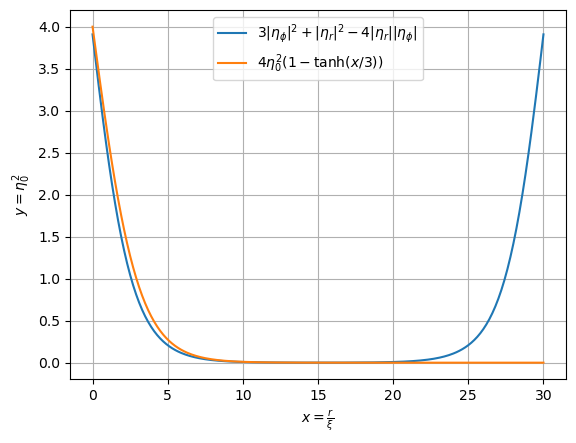
\includegraphics[width=0.6\textwidth]{../figures/numerator.png}
    \caption{Comparison of 
    $y=3\left(\eta^{(0)}_\phi\right)^2 + \left(\eta^{(0)}_r\right)^2-4\eta^{(0)}_r\eta^{(0)}_\phi$
    and $y=\eta_0^2\tanh(ax/\xi)$ for $a=1/3$ and $D=30\xi$.}
    \label{fig:numerator}
\end{figure}
\begin{figure}[h]
    \centering
    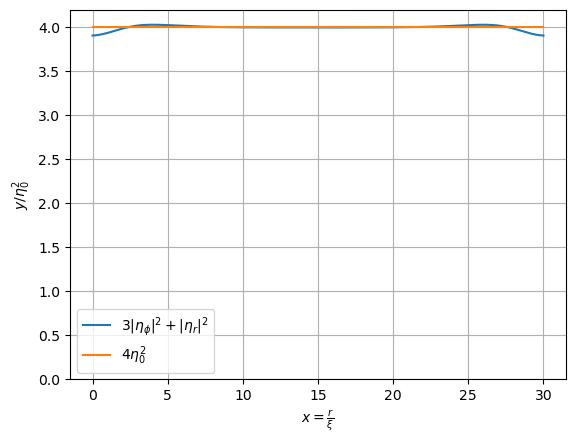
\includegraphics[width=0.6\textwidth]{../figures/denominator.png}
    \caption{Comparison of
    $y=3\left(\eta^{(0)}_\phi\right)^2 + \left(\eta^{(0)}_r\right)^2$
    and $y=4\eta_0^2$ for $D=30\xi$.}
    \label{fig:denominator}
\end{figure}

\section{London approximation}
We assume $\eta_i^{(m)}(r) = \eta_0$.
The angular momentum increase is
\begin{align}
    L_\pm(m) - L_\pm(m-1)
    =\frac{8M}{\hbar}\kappa_1\eta_0^2\pi\bigg[(R+D)^2-R^2\bigg]h
\end{align}
The free energy increase is
\begin{align}
    F_\pm(m)-F_\pm(m-1)=8\pi\kappa_1\eta_0^2\ln(\frac{R+D}{R})h(2m-1)
\end{align}
where $h$ is the thickness of the annulus. The critical angular velocity is
\begin{align}
    \Omega_m^\pm=\Omega_c\frac{\xi}{D}\frac{\ln{(1+D/R)}}{2+D/R}(2m-1),
\end{align}
where $\Omega_c = v_c/R$, $v_c = \hbar/M\xi$, $\xi^2=\kappa_1/|\alpha|$.
Actually, all of the GL parameters drop out
\begin{align}
    \Omega_m^\pm=\frac{\hbar}{MRD}\frac{\ln{(1+D/R)}}{2+D/R}(2m-1),
\end{align}
When $R\gg D$, we have
\begin{align}
    \Omega_m^\pm=\frac{\hbar}{MR^2}\left(m-\frac{1}{2}\right)
\end{align}
i.e.
\begin{align}
    \Omega_1=\frac{\hbar}{MR^2}\frac{1}{2}\qq{for}m=0\rightarrow m=1\\
    \Omega_2=\frac{\hbar}{MR^2}\frac{3}{2}\qq{for}m=1\rightarrow m=2\\
    \Omega_3=\frac{\hbar}{MR^2}\frac{5}{2}\qq{for}m=2\rightarrow m=3\\
    ...
\end{align}

\section{Numerical solution}

From the bulk free energy term we can get the bulk order parameter
$\eta_0 = \frac{1}{2}\sqrt\frac{|\alpha|}{\beta_1}$.
We also define the coherence length $\xi = \sqrt{\kappa_1/|\alpha|}$.

In weak-coupling limit, the GL equations in cylindrical basis are
\begin{align}
    \alpha\eta_k+2\beta_1\eta_i\eta_i^*\eta_k
    +\beta_1\eta_i^2\eta_k^*
    -\kappa_1\left(\partial_i^2\eta_k
    +\partial_k\partial_i\eta_i
    +\partial_j\partial_k\eta_j\right)\nonumber\\
    -\frac{\kappa_1}{r}\left[3\frac{\partial_\phi}{r}
    \left(\eta_r\delta_{k\phi}-\eta_\phi\delta_{kr}\right)+\partial_r\eta_k
    +2\partial_k\eta_r\right]\nonumber\\
    +\frac{\kappa_1}{r^2}\left[\eta_k+2\eta_r\delta_{kr}\right]=0.
\end{align}

The dimensionless GL equations in cylindrical basis are
\begin{align}
    -\eta_k+\frac{1}{2}\eta_i\eta_i^*\eta_k
    +\frac{1}{4}\eta_i^2\eta_k^*
    -(\partial_i^2\eta_k
    +\partial_k\partial_i\eta_i
    +\partial_j\partial_k\eta_j)\nonumber\\
    -\frac{1}{r}\left[3\frac{\partial_\phi}{r}
    \left(\eta_r\delta_{k\phi}-\eta_\phi\delta_{kr}\right)+\partial_r\eta_k
    +2\partial_k\eta_r\right]\nonumber\\
    +\frac{1}{r^2}\left[\eta_k+2\eta_r\delta_{kr}\right]=0.
\end{align}

The $r$ component of the GL equations is
\begin{align}
    -\eta_r+\frac{1}{2}\eta_i\eta_i^*\eta_r
    +\frac{1}{4}\eta_i^2\eta_r^*
    -(\partial_i^2\eta_r
    +\partial_r\partial_i\eta_i
    +\partial_j\partial_r\eta_j)
    -\frac{1}{r}\left[-3\frac{\partial_\phi}{r}\eta_\phi
    +3\partial_r\eta_r\right]
    +\frac{3}{r^2}\eta_r=0 \nonumber\\
    -\eta_r+\frac{1}{2}\eta_i\eta_i^*\eta_r
    +\frac{1}{4}\eta_i^2\eta_r^*
    -(\partial_i^2\eta_r
    +\partial_r\partial_i\eta_i
    +\partial_j\partial_r\eta_j)
    +3\left[\frac{1}{r^2}\partial_\phi\eta_\phi
    -\frac{1}{r}\partial_r\eta_r + \frac{\eta_r}{r^2}\right]=0 \nonumber\\
    -\eta_r+\frac{1}{2}\eta_i\eta_i^*\eta_r
    +\frac{1}{4}\eta_i^2\eta_r^*
    -3\partial_r^2\eta_r - \frac{1}{r^2}\partial_\phi^2\eta_r
    -\frac{2}{r}\partial_r\partial_\phi\eta_\phi
    +\frac{4}{r^2}\partial_\phi\eta_\phi
    -\frac{3}{r}\partial_r\eta_r + \frac{3}{r^2}\eta_r=0 \nonumber
\end{align}

The $\phi$ component of the GL equations is
\begin{align}
    -\eta_\phi+\frac{1}{2}\eta_i\eta_i^*\eta_\phi
    +\frac{1}{4}\eta_i^2\eta_\phi^*
    -\left(\partial_i^2\eta_\phi
    +\frac{\partial_\phi}{r}\partial_i\eta_i
    +\partial_j\frac{\partial_\phi}{r}\eta_j\right)
    -\frac{1}{r}\left[5\frac{\partial_\phi}{r}\eta_r
    +\partial_r\eta_\phi\right]
    +\frac{1}{r^2}\eta_\phi=0\nonumber\\
    -\eta_\phi+\frac{1}{2}\eta_i\eta_i^*\eta_\phi
    +\frac{1}{4}\eta_i^2\eta_\phi^*
    -3\frac{1}{r^2}\partial_\phi^2\eta_\phi
    -\partial_r^2\eta_\phi
    -\frac{2}{r}\partial_r\partial_\phi\eta_r
    -\frac{4}{r^2}\partial_\phi\eta_r
    -\frac{1}{r}\partial_r\eta_\phi
    +\frac{1}{r^2}\eta_\phi=0\nonumber
\end{align}

For the uniform flow approximation,
\begin{align}
    \bm{\eta}(r, \phi) = \left(\eta_r^{(n)}(r), \eta_\phi^{(n)}(r)\right) e^{in\phi}
\end{align}
which means that $\partial_\phi \rightarrow in$. We have
\begin{align}
    -\eta_r+\frac{1}{2}\eta_i\eta_i^*\eta_r
    +\frac{1}{4}\eta_i^2\eta_r^*
    -3\partial_r^2\eta_r + \frac{n^2}{r^2}\eta_r
    -\frac{2in}{r}\partial_r\eta_\phi
    +\frac{4in}{r^2}\eta_\phi
    -\frac{3}{r}\partial_r\eta_r + \frac{3}{r^2}\eta_r=0 \nonumber\\
    -\eta_\phi+\frac{1}{2}\eta_i\eta_i^*\eta_\phi
    +\frac{1}{4}\eta_i^2\eta_\phi^*
    +\frac{3n^2}{r^2}\eta_\phi
    -\partial_r^2\eta_\phi
    -\frac{2in}{r}\partial_r\eta_r
    -\frac{4in}{r^2}\eta_r
    -\frac{1}{r}\partial_r\eta_\phi
    +\frac{1}{r^2}\eta_\phi=0\nonumber
\end{align}
We ignore the $(n)$ superscript for the sake of simplicity.
The solutions of $n=1$ may corresponds to the
$(p_x + ip_y, m=0)$ state, or the $(p_x - ip_y, m=2)$ state.

\section{Large flow}

When the flow field is large, we denote the superfluid flow field at the inner radius as
$v_s = \frac{\hbar}{MR}\partial_\phi\theta$, and
\begin{align}
    \bm{\eta}(r, \phi, v_s)
    = \bm{\eta}^{(n)}(r) e^{in\phi} = \bm{\eta}(r, v_s)e^{i(\partial_\phi\theta)\phi}
    = \bm{\eta}(r, v_s)e^{i\frac{v_s R}{v_c \xi}\phi}
\end{align}
where the critical flow field $v_c = \hbar/M\xi$ and $\xi^2=\kappa_1/|\alpha|$.
We also have $n=\frac{v_s}{v_c}\frac{R}{\xi}$.

\section{Cartesian basis}

In Cartesian basis, weak-coupling limit dimensionless GL equations are
\begin{align}
    -\eta_k+\frac{1}{2}\eta_i\eta_i^*\eta_k
    +\frac{1}{4}\eta_i^2\eta_k^*-\left(\partial_i^2\eta_k
    +\partial_k\partial_i\eta_i
    +\partial_j\partial_k\eta_j\right) = 0
\end{align}
The $x$ component of the GL equations is
\begin{align}
    -\eta_x+\frac{3}{4}\eta_x^2\eta_x^*
    +\frac{1}{2}\eta_y\eta_y^*\eta_x
    +\frac{1}{4}\eta_y^2\eta_x^*
    -3\partial_x^2\eta_x - \partial_y^2\eta_x
    -2\partial_y\partial_x\eta_y = 0
\end{align}
The $y$ component of the GL equations is
\begin{align}
    -\eta_y+\frac{3}{4}\eta_y^2\eta_y^*
    +\frac{1}{2}\eta_x\eta_x^*\eta_y
    +\frac{1}{4}\eta_x^2\eta_y^*
    -3\partial_y^2\eta_y - \partial_x^2\eta_y
    -2\partial_x\partial_y\eta_x = 0
\end{align}
\end{document}
